\hypertarget{ch4}{%
\chapter{Towards a multisensor optical-radar approach for snow water equivalent retrievals}\label{ch4}}

%==============================================================================
%==============================================================================
%==============================================================================

\hypertarget{ch4-abstract}{\section{Abstract}\label{ch4-abstract}}


%==============================================================================
%==============================================================================
%==============================================================================
\hypertarget{ch4-intro}{\section{Introduction}\label{ch4-intro}}



Measuring the spatial and temporal distribution of snow water equivalent (SWE) and snow depth in the world’s mountains is the preeminent unsolved challenge facing snow hydrology \citep{dozierEstimatingSpatialDistribution2016}. Despite the critical importance of these measurements, no single spaceborne sensor will be able to monitor SWE from all snow classes \citep{sturmSeasonalSnowCover1995, sturmRevisitingGlobalSeasonal2021} globally at scales relevant to basin-scale water resource management \citep{lettenmaierInroadsRemoteSensing2015}. Thus, breakthroughs in spaceborne SWE monitoring will require a multisensor approach \citep{durandAchievingBreakthroughsGlobal2021}, also known as sensor fusion, with the combination of optical and synthetic aperture radar (SAR) as a prime candidate. SAR will be at the forefront of future advancements in satellite remote sensing of SWE and snow depth, with multiple snow-focused SAR missions under development from NASA and the Canadian Space Agency (CSA) \citep{tsangReviewArticleGlobal2022, yuehSatelliteSyntheticAperture2021, garnaudQuantifyingSnowMass2019}. In addition, there are planned launches of L-band SARs such as the NASA-ISRO SAR (NISAR) in 2024 and the European Space Agencies (ESA) Radar Observation System for Europe in L-band (ROSE-L) near the end of the decade. L-band interferometric SAR (InSAR) shows promise for SWE change monitoring \citep{tarriconeEstimatingSnowAccumulation2023a, marshallLBandInSARDepth2021, naglerAirborneExperimentInsar2022}. Moreover, the launch of Sentinel-1C in 2023 reestablishes the two-satellite constellation and continues global C-band coverage (***rework this sentence***).  \par


%%%%: topic: reviewing SAR-based dry snow cover algorithms and showing they're not sufficient
Snowpack that is important for water resources mainly exists in complex mid-latitude mountain environments (cite). In the WUS, snow covered area (SCA) ranges between a median value of $\sim$3,000 km$^{2}$ at its summer minimum and $\sim$10$^{6}$ km$^{2}$ during the winter maximum \citep{rittgerSnowToday2022} (more here, possibly percentage of land area). Existing SAR-based techniques do not possess the capability to accurately delineate dry snow cover on their own \citep{tsaiRemoteSensingSnow2019}. There have been experimental attempts to use SAR at various frequencies and polarizations to detect dry (add varade) snow \citep{rottThematicStudiesAlpine1994, shiMappingSeasonalSnow1997}. Many studies employed a complex polarimetric decomposition (sen1 dual pol) (cite) or machine learning techniques (cite). While there has been progress in this area, none of these methods are mature enough for operational snow cover mapping. \par

%%%% topic: a review of current operational snow cover products
Contrarily, methods for passive microwave (PM), optical, and near-infrared (NIR) snow cover mapping are mature and routinely practiced \citep{dozierMultispectralHyperspectralRemote2004,saberiReviewSnowWater2020}. PM instruments produce data on the spatial scale of tens of kilometers, are only effective in dry snowpacks $<$ 1 m, and therefore are not suitable for mountain watershed snowpack applications (more citations here). Optical and NIR snow mapping methods date back to the earliest earth-observing satellites \citep{rangoSatellitePotentialsSnowcover1976a}. Numerous studies have utilized multi-spectral data in mountain environments from the Landsat 5-9 \citep{dozierSpectralSignatureAlpine1989} (more) and the Moderate Resolution Imaging Spectroradiometer (MODIS) \citep{painterRetrievalSubpixelSnowcovered2003, painterRetrievalSubpixelSnow2009, rittgerAssessmentMethodsMapping2013} (***rework, good start***). 

These optical methods are the basis for various snow cover products. In the western US (WUS), there is a fractional snow covered area (fSCA) product from Landsat 8/9 \citep{selkowitzUSGSLandsatSnow2017}, and a Normalized Snow Difference Index (NDSI) \citep{dozierSpectralSignatureAlpine1989, hallDevelopmentMethodsMapping1995} product from the MODIS \citep{hallMODISSnowcoverProducts2002} and the Visible Infrared Imaging Radiometer Suite (VIIRS) \citep{justiceLandCryosphereProducts2013}. For Europe and various other parts of the world, Gascoin et al. \citep{gascoinTheiaSnowCollection2019a} created the Theia Snow collection, which uses Landsat 8 and Sentinel 2 A/B independently to map binary snow presence.

%%%% topic: lidar from space won't work
Previous research has explored various types of multisensor approaches for different snow monitoring applications. The Airborne Snow Observatory (ASO) \citep{painterAirborneSnowObservatory2016} leverages suborbital lidar altimetry \citep{deemsLidarMeasurementSnow2013}, hyperspectral imaging \citep{nolinMappingAlpineSnow1993}, and spatially distributed snow density modeling \citep{marksSpatiallyDistributedEnergy1999} to estimate basin-scale SWE at high resolutions (1--50 m). While this technique is now operational, there is no clear pathway to space for spatially distributed lidar retrievals. Currently, only linear transects from satellites such as NASA's Ice, Cloud and Land Elevation Satellite-2 (ICESat-2) \citep{abdalatiICESat2LaserAltimetry2010} and the Global Ecosystem Dynamics Investigation (GEDI) \citep{dubayahGlobalEcosystemDynamics2020} are possible. Moreover, even the sparse measurements from the aforementioned spaceborne lidars show uncertainties of 1--2 m for snow depth retrievals in complex terrain \citep{enderlinUncertaintyICESat2ATL062022, deschamps-bergerEvaluationSnowDepth2022}. \par

%%%% topic: optical fusion
*** Recently, NASA released the Harmonized Landsat and Sentinel-2 (HLS) data product which fuses the two sensors to produce lower temporal resolution surface reflectance data.
Rittger et al. \citep{rittgerMultisensorFusionUsing2021} combined Landsat and MODIS with machine learning to achieve a spatiotemporally complete 30 m fSCA dataset over the Sierra Nevada Mountains, CA. ****

%%%% topic: SAR/optical for SWE or depth fusion products
Few studies have employed optical and SAR data synergistically for snow depth and SWE retrievals. Lievens et al. \citep{lievensSnowDepthVariability2019,lievensSentinel1SnowDepth2022} developed a Sentinel-1 C-band snow depth retrieval algorithm using the co-polarized and cross-polarized backscatter ratio. They identified snow cover using 1 km$^{2}$ binary snow cover information from the Interactive Multisensor Snow and Ice Mapping System (IMS) \citep{u.s.nationalicecenterIMSDailyNorthern2008, ramsayInteractiveMultisensorSnow1998, helfrichEnhancementsForthcomingDevelopments2007}, and fractional forest cover using the 1 km$^{2}$ global consensus land cover dataset \citep{tuanmuGlobal1kmConsensus2014}, at both European and Northern Hemispherical scales. These new methods are promising, especially as the physical mechanisms governing the retrievals continue to emerge \citep{zhuModelingScatteringDense2023}. \cite{tarriconeEstimatingSnowAccumulation2023a} utilized Landsat fSCA information with UAVSAR L-band InSAR data to estimate both snow ablation and accumulation in the Jemez Mountains, NM. They note the multifaceted importance of a multisensor approach for snow cover delineation and SAR atmospheric correction. \par

These past studies have subjectively selected various products (e.g., fSCA, binary, NSDI), spatial resolutions ($\sim$ 1--1000 m), and temporal resolutions (1--16 d) without any systematic investigation of the uncertainties associated with each one. Our study aims to better understand the variability between common snow cover data products and how that uncertainty propagates into SAR-based SWE retrieval techniques. To do this, we analyze L-band InSAR SWE changes estimates from Uninhabited Aerial Vehicle Synthetic Aperture Radar (UAVSAR) collected by the NASA SnowEx 2020 \cite{marshallNASASnowEx20202019} campaign in the Upper San Joaquin (USJ) River basin in Sierra Nevada Mountains, CA. NISAR's upcoming launch in early 2024 makes the InSAR approach the most ***time sensitive*** of the SWE measurement techniques.

% -Despite the previously stated importance of a multisensor snow depth and SWE monitoring approach, few works have explored the best combination of sensors.
% - Herein, we will refer to our methodology as a ``multisensor" approach. Previous works (karl, add others) have used the term ``sensor fusion", which can be thought of as the same thing. Neither of these terms has concrete definitions, and therefore our word choice is subjective.


%==============================================================================
%%%%%%%%%%%%%%%%%%%%%%%%%%%%%%%%%%%%%%%%%%%%%%%%%%%%%%%%%%%%%%%%%%%%%%%%%%%%%%%%
\hypertarget{ch4-methods}{\section{Data Overview}\label{ch4-methods}}
In this section, we overview the UAVSAR data and the six different SCA products analyzed within this study.

%%%%%%%%%%%%%%%%%%%%%%%%%%%%%%%%%%%%%%%%%%%%%%%%%%%%%%%%%%%%%%%%%%%%%%%%%%%%%%%%
\hypertarget{ch4-methods-1}{\subsection{UAVSAR}\label{ch4-methods-1}}

UAVSAR flights occurred on 26 February 2020 and 11 March 2011 2020 and covered an area of $\sim$1600 km$^{2}$. These data were processed by the UAVSAR team at NASA's Jet Propulsion Laboratory (JPL) to create a single 14 d baseline 6 m ground projected InSAR pair. These products include unwrapped phase (herein referred to as phase), coherence, and incidence angle. The reader is referred to the supplementary material for information on UAVSAR on specific processing parameters. To better replicate the NISAR returns, we resampled the 6 m UAVSAR data to 80 m, which is the resolution NISAR data products will be produced. To do this, we used Sentinel-1 Geocoded Unwrapped Interferograms (S1 GUNW), produced in the same data format and spatial resolution (80 m) that NISAR data will be. These data are generated by NASA's Advanced Rapid Imaging and Analysis (ARIA) \citep{bekaertDevelopmentDisseminationStandardized2019,buzzangaSustainedMonitoringSubsidence2020} project and accessed via the Alaska Satellite Facility Distributed Active Archive Center (ASF DAAC).


\begin{figure}[ht]
\includegraphics[width=13cm]{figures/ch4_figs/data_section_plot_v3.png}
\centering
\caption{UAVSAR \textbf{(a)} coherence, \textbf{(b)} phase, \textbf{(c)} incidence angle from the 2/26--3/11 InSAR pair. The grey pixels in \textbf{(b)} are pixels lost in the unwrapping process, which is caused by low coherence values. The full extent of S-NISAR \textbf{(d)} phase and \textbf{(e)} coherence from the 2/22--3/05 InSAR pair. The USJ watershed boundary and UAVSAR swath are shown by black lines, with Lake Tahoe represented by the blue in the top left corner. The black dotted line is a 1500 m contour approximating the seasonal snow zone.}
\end{figure}
\clearpage

\begin{table}[t]
\centering
\caption{Technical specifications of the UAVSAR L-band radar (top). InSAR processing and data parameters of the 26 February--11 March UAVSAR InSAR pair (bottom).}
\begin{tabular}{ll}
\toprule Parameter & Value \\
\midrule
Wavelength & 23.84\,cm \\
Frequency & 1.26\,GHz \\
Polarization & Quad pol \\
Bandwidth & 80\,MHz \\
Pulse length & 40\,$\mu$s \\
Radar look direction & Left \\
Range swath width & 22\,km \\
Average near-range look angle & 28.01$^{\circ}$\\
Average far-range look angle & 68.9$^{\circ}$\\
\midrule
Ground range pixel spacing & 80\,m \\
Number of looks in range & 3 \\
Number of looks in azimuth & 12 \\
Phase unwrapping method & ICU \\
Phase unwrapping filtering method & Low pass \\
Phase unwrapping filter window size & 3~pixels\,$\times$\,3~pixels \\
\bottomrule
\end{tabular}
\end{table}


%%%%%%%%%%%%%%%%%%%%%%%%%%%%%%%%%%%%%%%%%%%%%%%%%%%%%%%%%%%%%%%%%%%%%%%%%%%%%%%%
\hypertarget{ch4-methods-2}{\subsection{Snow cover data}\label{ch4-methods-2}}

Snow cover data is derived from the normalized snow difference index (NDSI) \citep{dozierSpectralSignatureAlpine1989} or spectral-mixture analysis 

\begin{equation}
NDSI = \frac{{R_{VIS,\lambda} - R_{SWIR,\lambda}}}{{R_{VIS,\lambda} + R_{SWIR,\lambda}}}
\end{equation}


\begin{figure}[h]
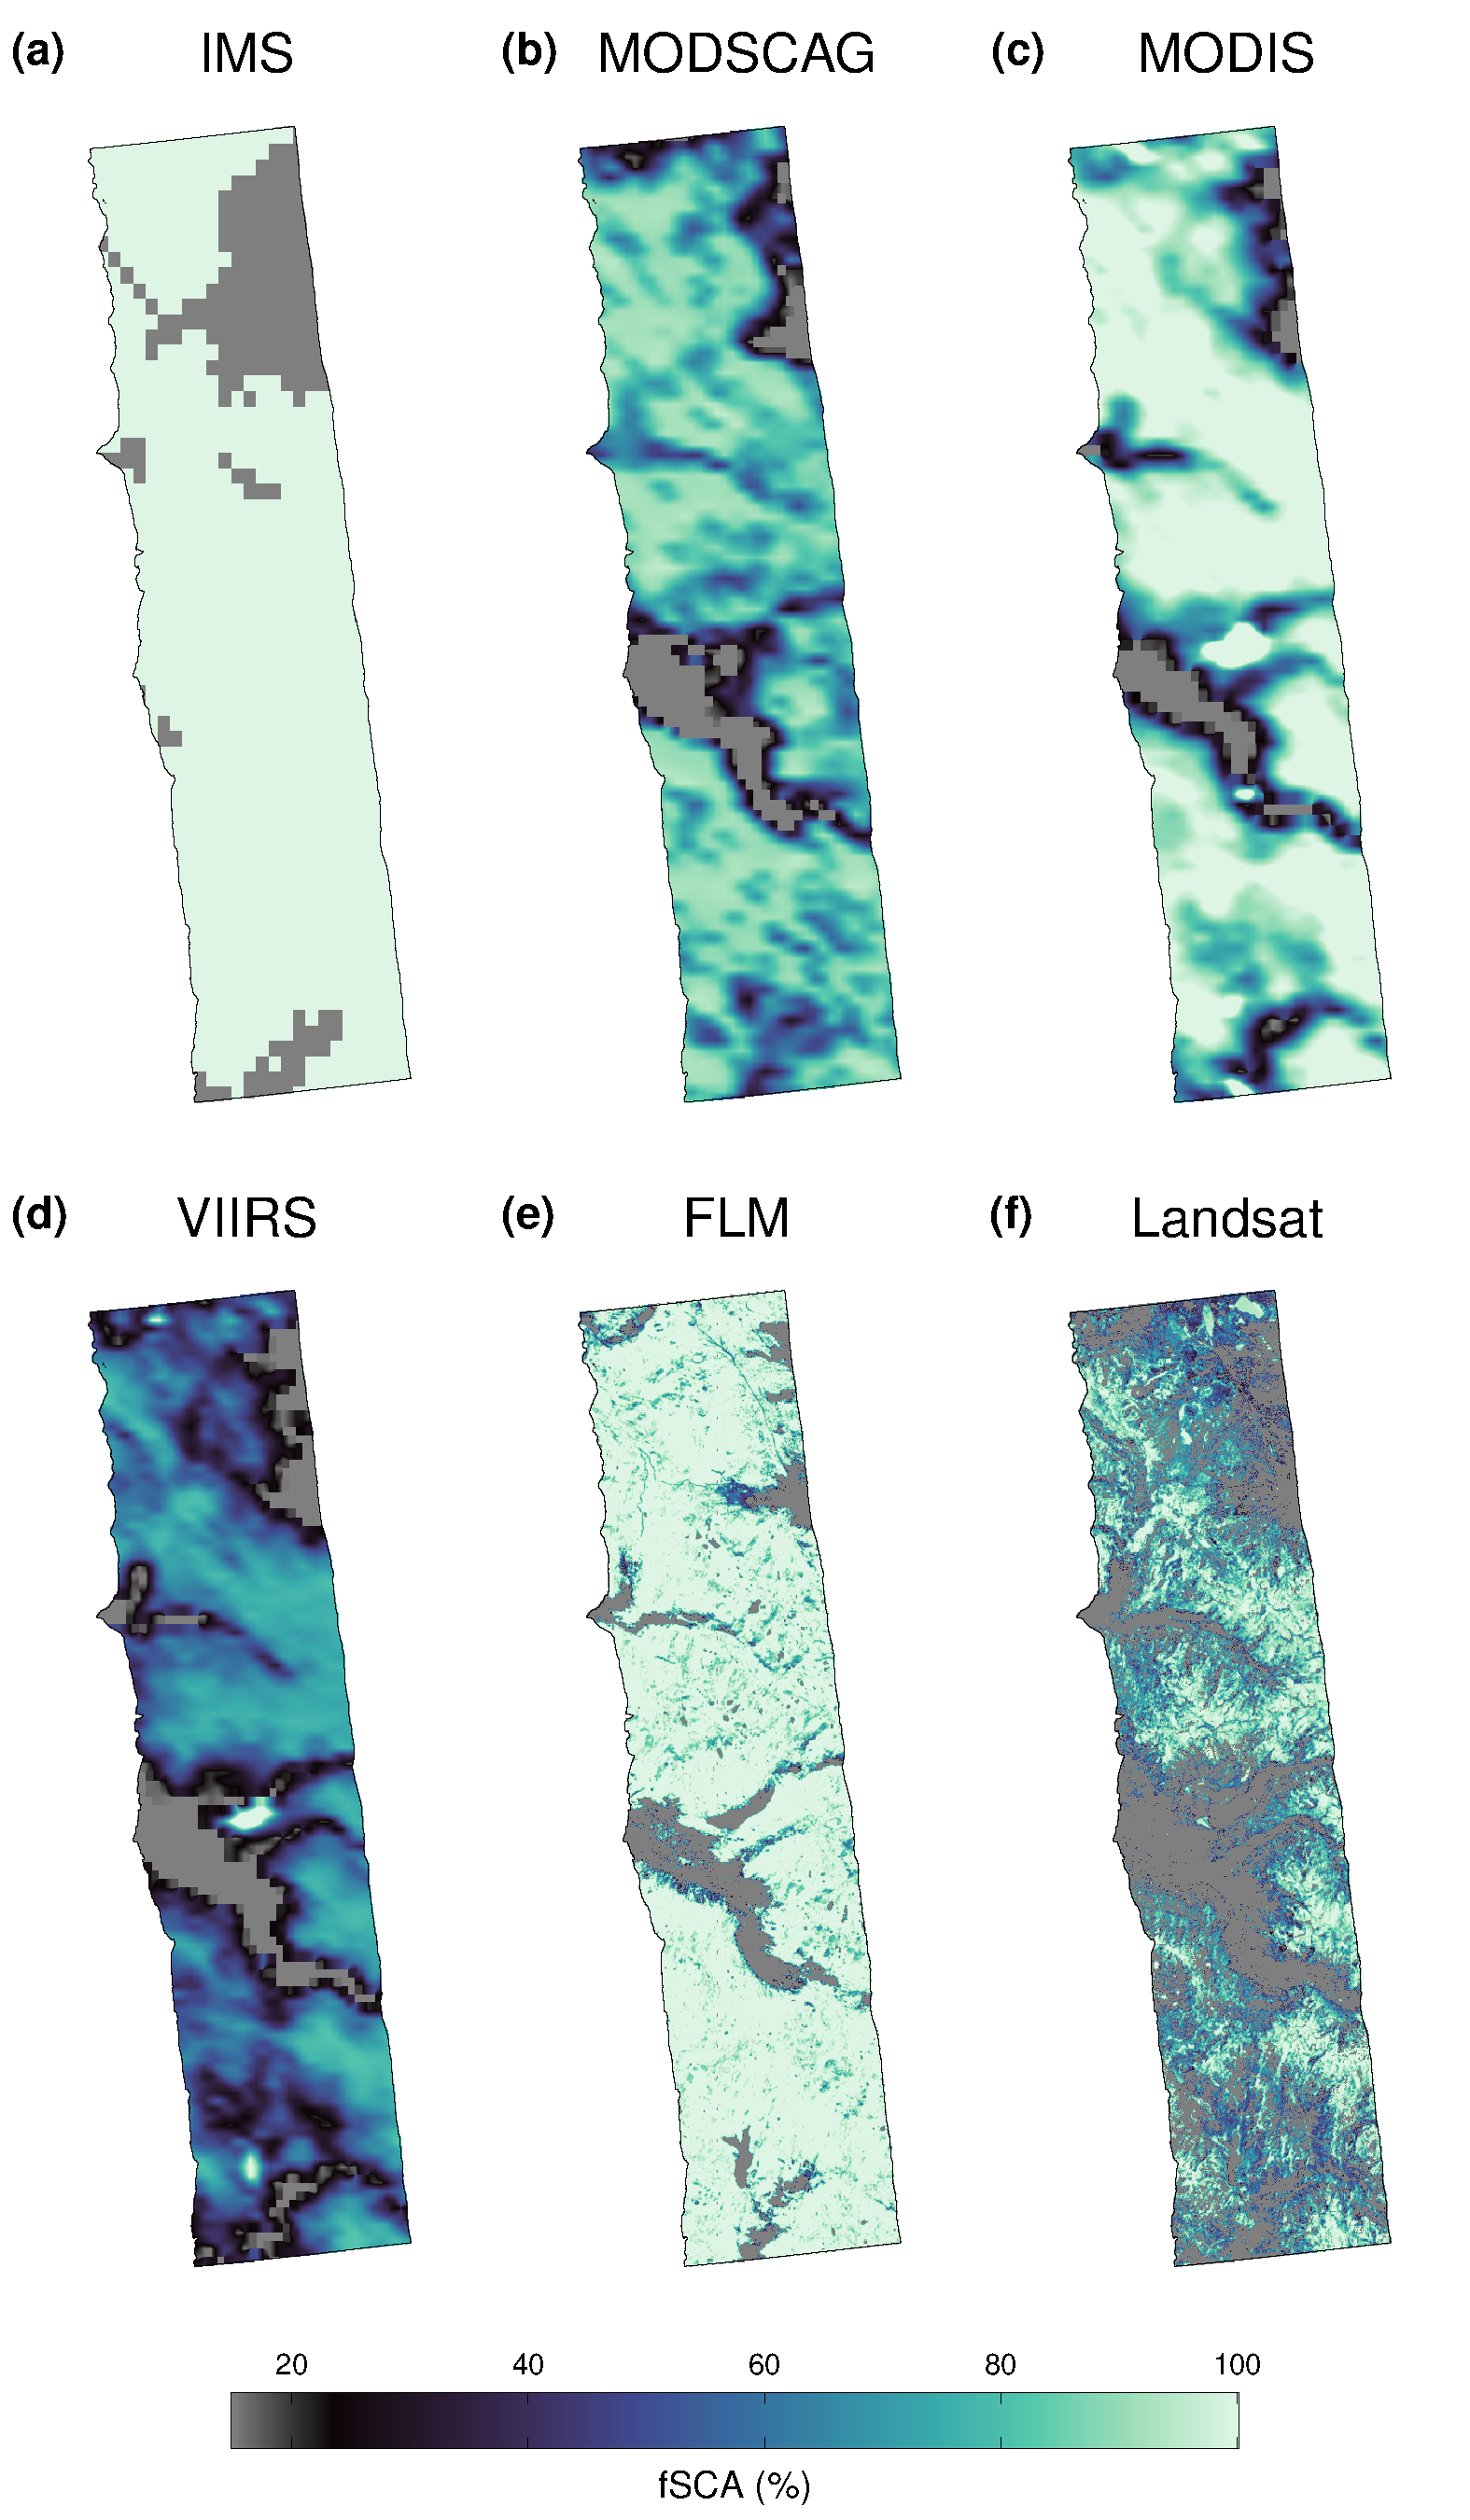
\includegraphics[width=\textwidth]{figures/ch4_figs/fsca_usvar_v2.pdf}
\caption{fSCA from \textbf{(a)} IMS, \textbf{(b)} MODSCAG, \textbf{(c)} MODIS, \textbf{(d)} VIIRS, \textbf{(e)} FLM, and \textbf{(f)} Landsat. The dark gray represents areas with < 15 \% fSCA}
\end{figure}
\clearpage
%%%%%%%%%%%%%%%%%%%%%%%%%%%%%%%%%%%%%%%%%%%%%%%%%%%%%%%%%%%%%%%%%%%%%%%%%%%%%%%%
\hypertarget{ch4-methods-3}{\subsubsection{IMS}\label{ch4-methods-3}}


The National Oceanic and Atmospheric Administration’s National Environmental Satellite Data and Information Service (NOAA/NESDIS) Interactive Multisensor Snow and Ice Mapping System (IMS) is a hemispherical scale binary 1 km snow cover product originally created to help with numerical weather prediction 
\citep{ramsayInteractiveMultisensorSnow1998, helfrichEnhancementsForthcomingDevelopments2007}. The input data comes a variety of platforms, including but not limited to: the National Oceanic and Atmospheric Administration's (NOAA's) next generation of geostationary satellites (GOES) constellation \citep{menzelIntroducingGOESIFirst1994}, the Advanced Very High Resolution Radiometer (AVHRR) \citep{cracknellAdvancedVeryHigh1997}, MODIS \citep{salomonsonMODISAdvancedFacility1989}, and the National Operational Hydrologic Remote Sensing Center (NOHRSC) SNOw Data Assimilation System (SNODAS) \citep{barrettandrewNationalOperationalHydrologic2003}.

%%%%%%%%%%%%%%%%%%%%%%%%%%%%%%%%%%%%%%%%%%%%%%%%%%%%%%%%%%%%%%%%%%%%%%%%%%%%%%%%
\hypertarget{ch4-methods-4}{\subsubsection{MODSCAG}\label{ch4-methods-4}}


The MODIS Snow-Covered Area and Grain size (MODSCAG) \citep{painterRetrievalSubpixelSnow2009} is a spectral-mixing model that uses various end-members (e.g. rock, soil, snow, clouds, etc.) to produce estimates of fSCA, fractional vegetation (fVEG), snow grain size, and albedo.


%%%%%%%%%%%%%%%%%%%%%%%%%%%%%%%%%%%%%%%%%%%%%%%%%%%%%%%%%%%%%%%%%%%%%%%%%%%%%%%%
\hypertarget{ch4-methods-5}{\subsubsection{MODIS}\label{ch4-methods-5}}

The MODIS cloud-gap-filled (CGF) snow cover product \citep{hallEvaluationMODISVIIRS2019} provides daily NSDI values at 500 m spatial resolution from the Terra (MOD10A1F) and Aqua (MYD10A1F) satellites. These


\hypertarget{ch4-methods-6}{\subsubsection{VIIRS}\label{ch4-methods-6}}

The Visible Infrared Imaging Radiometer Suite (VIIRS) on the Suomi National Polar Partnership (S-NPP) produces a daily CGF NDSI product at 375 m spatial resolution \citep{hallEvaluationMODISVIIRS2019}.

\hypertarget{ch4-methods-7}{\subsubsection{FLM}\label{ch4-methods-7}}

The fused Landsat-MODIS (FLM) product created by \cite{rittgerMultisensorFusionUsing2021}

\hypertarget{ch4-methods-8}{\subsubsection{Landsat fSCA}\label{ch4-methods-8}}

Landsat~8 fSCA \citep{u.s.geologicalsurveyearthresourcesobservationandsciencecenterCollection1LandsatLevel32018} data from 4~March 2020 (Fig.~4.2e). These data are generated using a spectral unmixing analysis based on the MODSCAG algorithm developed for MODIS (Painter et al., 2009). The data processing workflow includes water masking, cloud masking, and canopy cover corrections \citep{selkowitzUSGSLandsatSnow2017, stillingerLandsatMODISVIIRS2023}. As of 2021 (**check this), the data products include both viewable fSCA and total ground fSCA. To estimate total fSCA in areas with canopy cover, a moving window analysis algorithm is employed, and it selects 


% Within the full UAVSAR swath, 29.7\,\% of pixels were entirely snow-free on 18~February (Fig.~3.4a), increasing to 38.1\,\% on 5~March (Fig.~3.4b). For just the study area, 4.1\,\% of pixels were snow-free on 18~February (Fig.~3.4d), with an increase to 9.1\,\% by 5~March (Fig.~3.4e).

\hypertarget{ch4-methods-8}{\subsection{In situ snow data}\label{ch4-methods-8}}

Snow pit from the SnowEx campaign
CADWR pillows -- name them

\hypertarget{ch4-methods}{\section{Methods}\label{ch4-methods}}
\hypertarget{ch4-methods}{\subsection{InSAR}\label{ch4-methods}}
%==============================================================================
\hypertarget{ch4-results}{\section{Results}\label{ch4-results}}
\hypertarget{ch4-results}{\subsection{$\Delta$SWE Estimates}\label{ch4-results}}

\hypertarget{ch4-results}{\subsection{$\Delta$SWE Variability}\label{ch4-results}}

Variability arises from various sources

\begin{figure}[t]
\centering
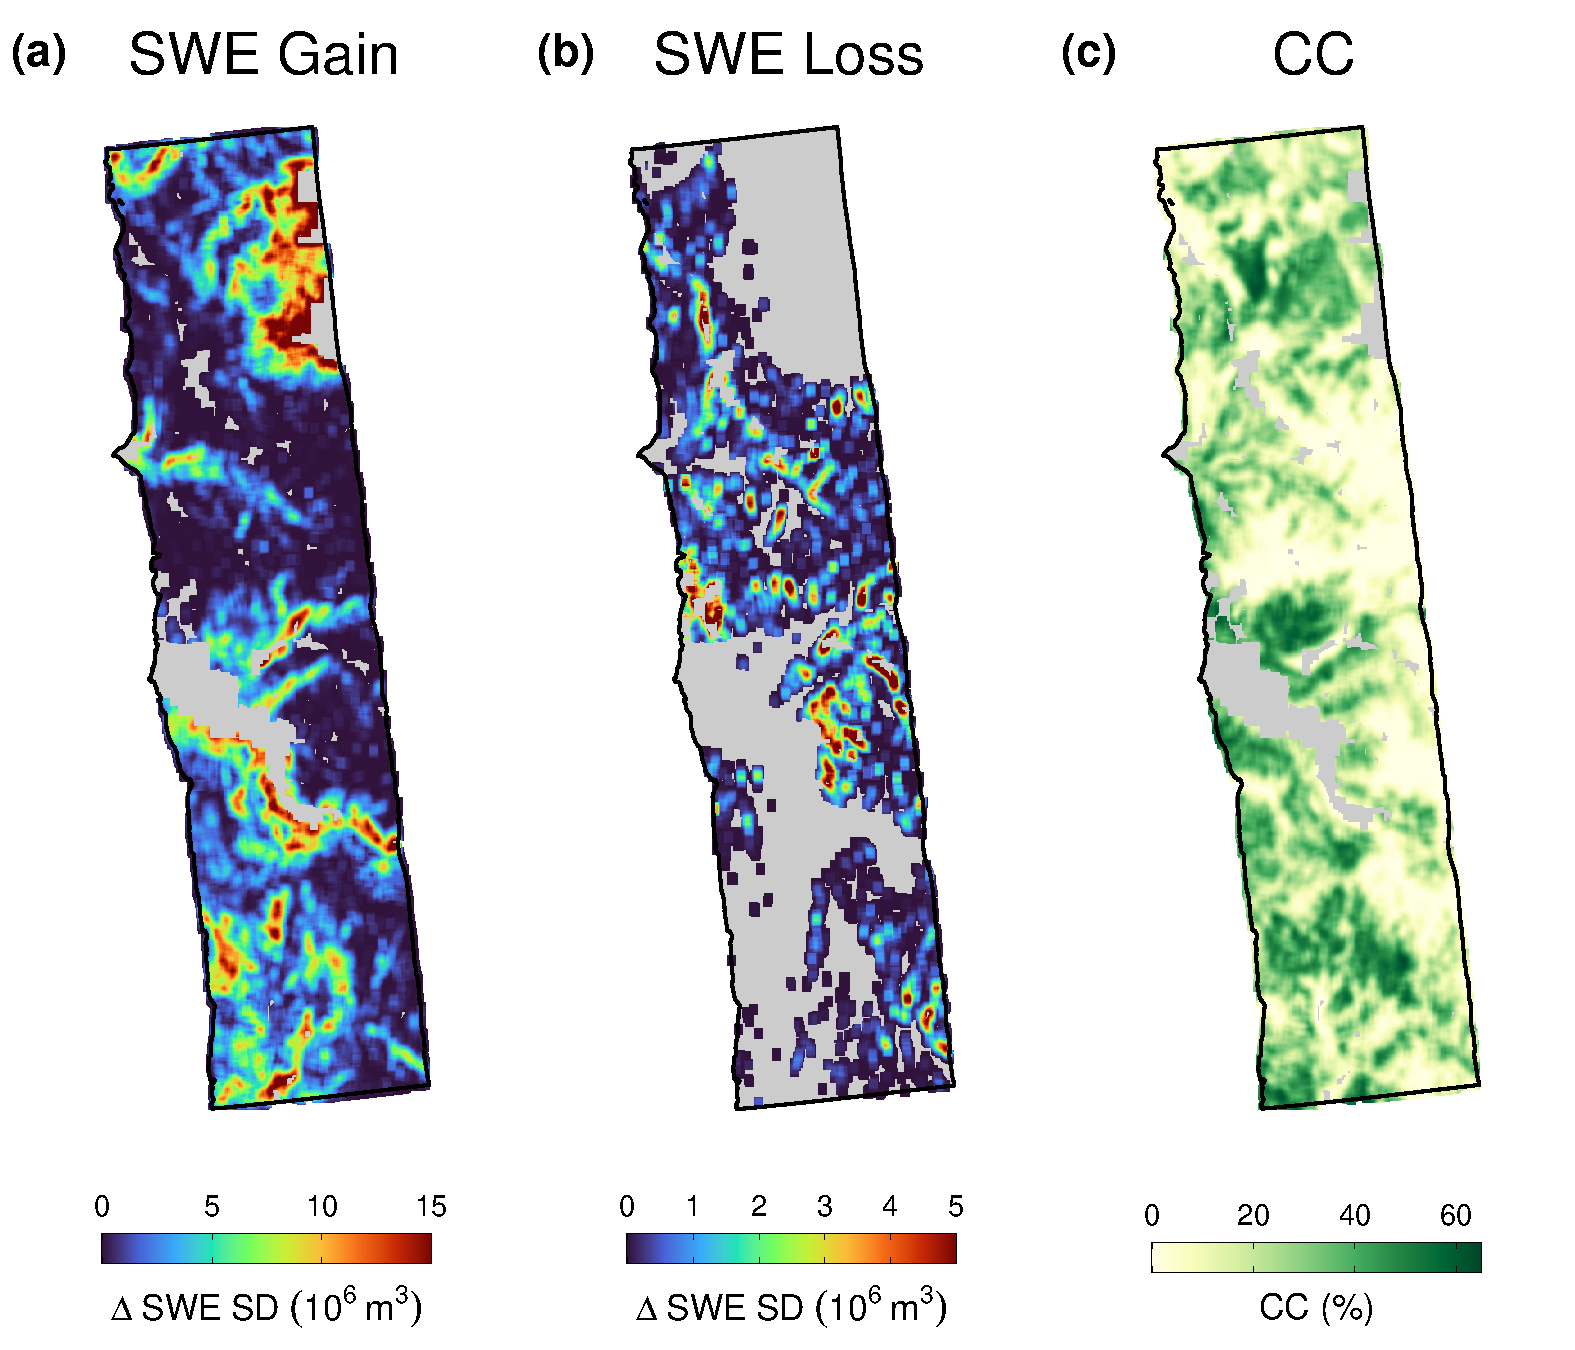
\includegraphics[width=\textwidth]{figures/ch4_figs/sd_vs_cc_map_v3.pdf}
\centering
\caption{Showing SD for blahhhh}
\end{figure}

\begin{figure}[t]
\centering
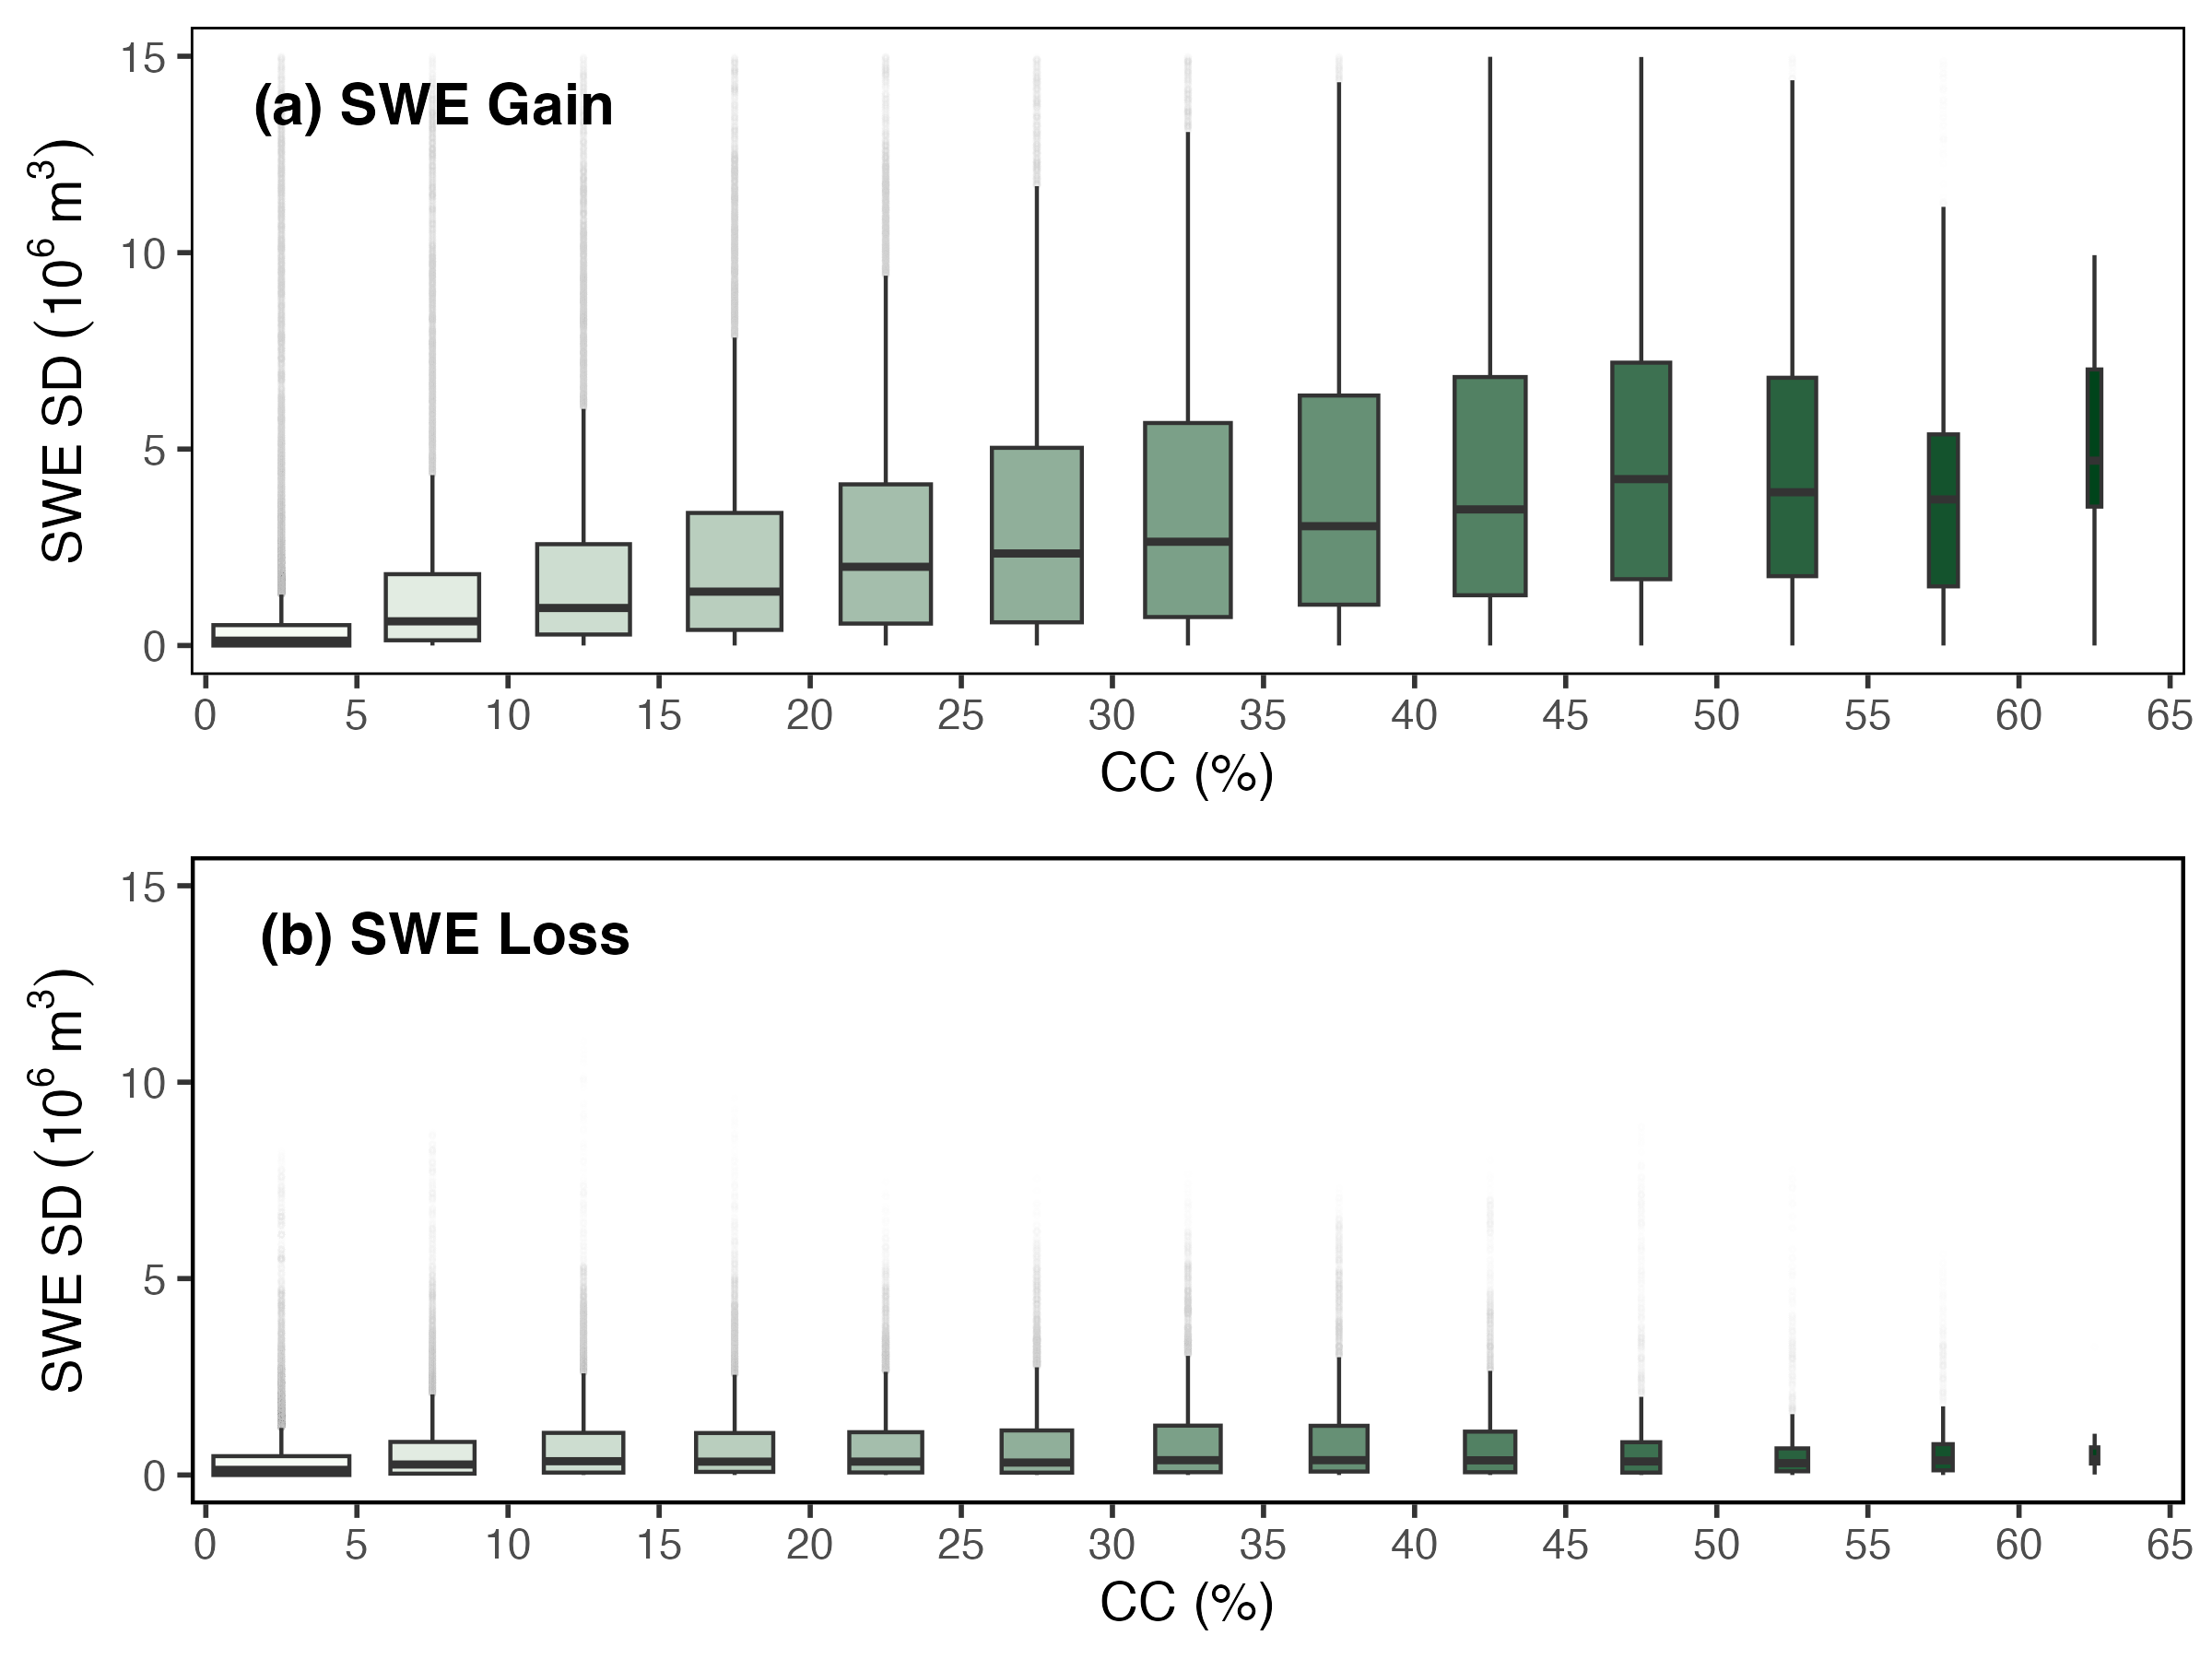
\includegraphics[width=\textwidth]{figures/ch4_figs/swe_sd_bp_v4.png}
\centering
\caption{Boxplots showing the relationship between CC \% SWE SD for \textbf{(a)} gain and \textbf{(b)} loss.}
\end{figure}

%==============================================================================
%==============================================================================
%==============================================================================
\hypertarget{ch5-discussion}{\section{Discussion}\label{ch4-discussion}}

-Paragraph on the need to incorporate Very-High-Resolution (VHR) commercial satellite imagery: sources are \citep{huImprovingMountainSnow2022, thalerEstimatingSnowCover2023,yangHighresolutionMappingSnow2023,johnHighResolutionSnowCoveredArea2022}

%==============================================================================
%==============================================================================
%==============================================================================
\hypertarget{ch6-conclusions}{\section{Conclusions}\label{ch6-conclusions}}




\bibliographystyle{apalike}
\bibliography{ch4.bib}
